
%!TEX root = ../main.tex

\chapter{Grundlagen verwendeter Technologien}
Um eine Lösung für die geschilderte Problemstellung zu erarbeiten, ist ein
Verständnis verschiedener Technologien erforderlich. Diese Grundlagen werden in diesem Kapitel benannt
und erläutert.


\section{Mikrocontroller}
Ein Mikrocontroller ist ein elektronisches Bauteil, das auf einem einzigen Chip integriert ist und die Funktionen
eines Prozessors, Speichers und digitaler Ein- und Ausgabepins vereint. Mikrocontroller werden häufig in eingebetteten
Systemen eingesetzt, um Steuerungs- und Verarbeitungsaufgaben auszuführen. Sie finden Anwendung in einer Vielzahl von
Bereichen, von Consumer-Elektronik bis hin zu medizinischen Geräten.

Ein typischer Mikrocontroller besteht aus mehreren Hauptkomponenten:
\begin{itemize}
    \item \textbf{\ac{CPU}:} Dies ist das Herzstück des Mikrocontrollers, das für die
          Ausführung von Befehlen und die Verarbeitung von Daten verantwortlich ist.
    \item \textbf{Speicher:} Mikrocontroller enthalten sowohl programmierbaren Speicher (\ac{ROM} oder Flash) für die
          Speicherung von Programmen als auch \ac{RAM} für temporäre Datenhaltung.
    \item \textbf{Peripheriegeräte:} Mikrocontroller verfügen über verschiedene eingebaute Peripheriegeräte wie Timer,
          Zähler, A/D- und D/A-Wandler, Kommunikationsschnittstellen (\ac{UART}, \ac{SPI}, \ac{I2C}) und \ac{GPIO}-Pins
          zur Interaktion mit der Umgebung.
    \item \textbf{Taktgenerator:} Dieser erzeugt die Taktsignale, die die Geschwindigkeit der \ac{CPU} und anderer
          Komponenten des Mikrocontrollers steuern.
\end{itemize}

\begin{figure}[H]
    \centering
    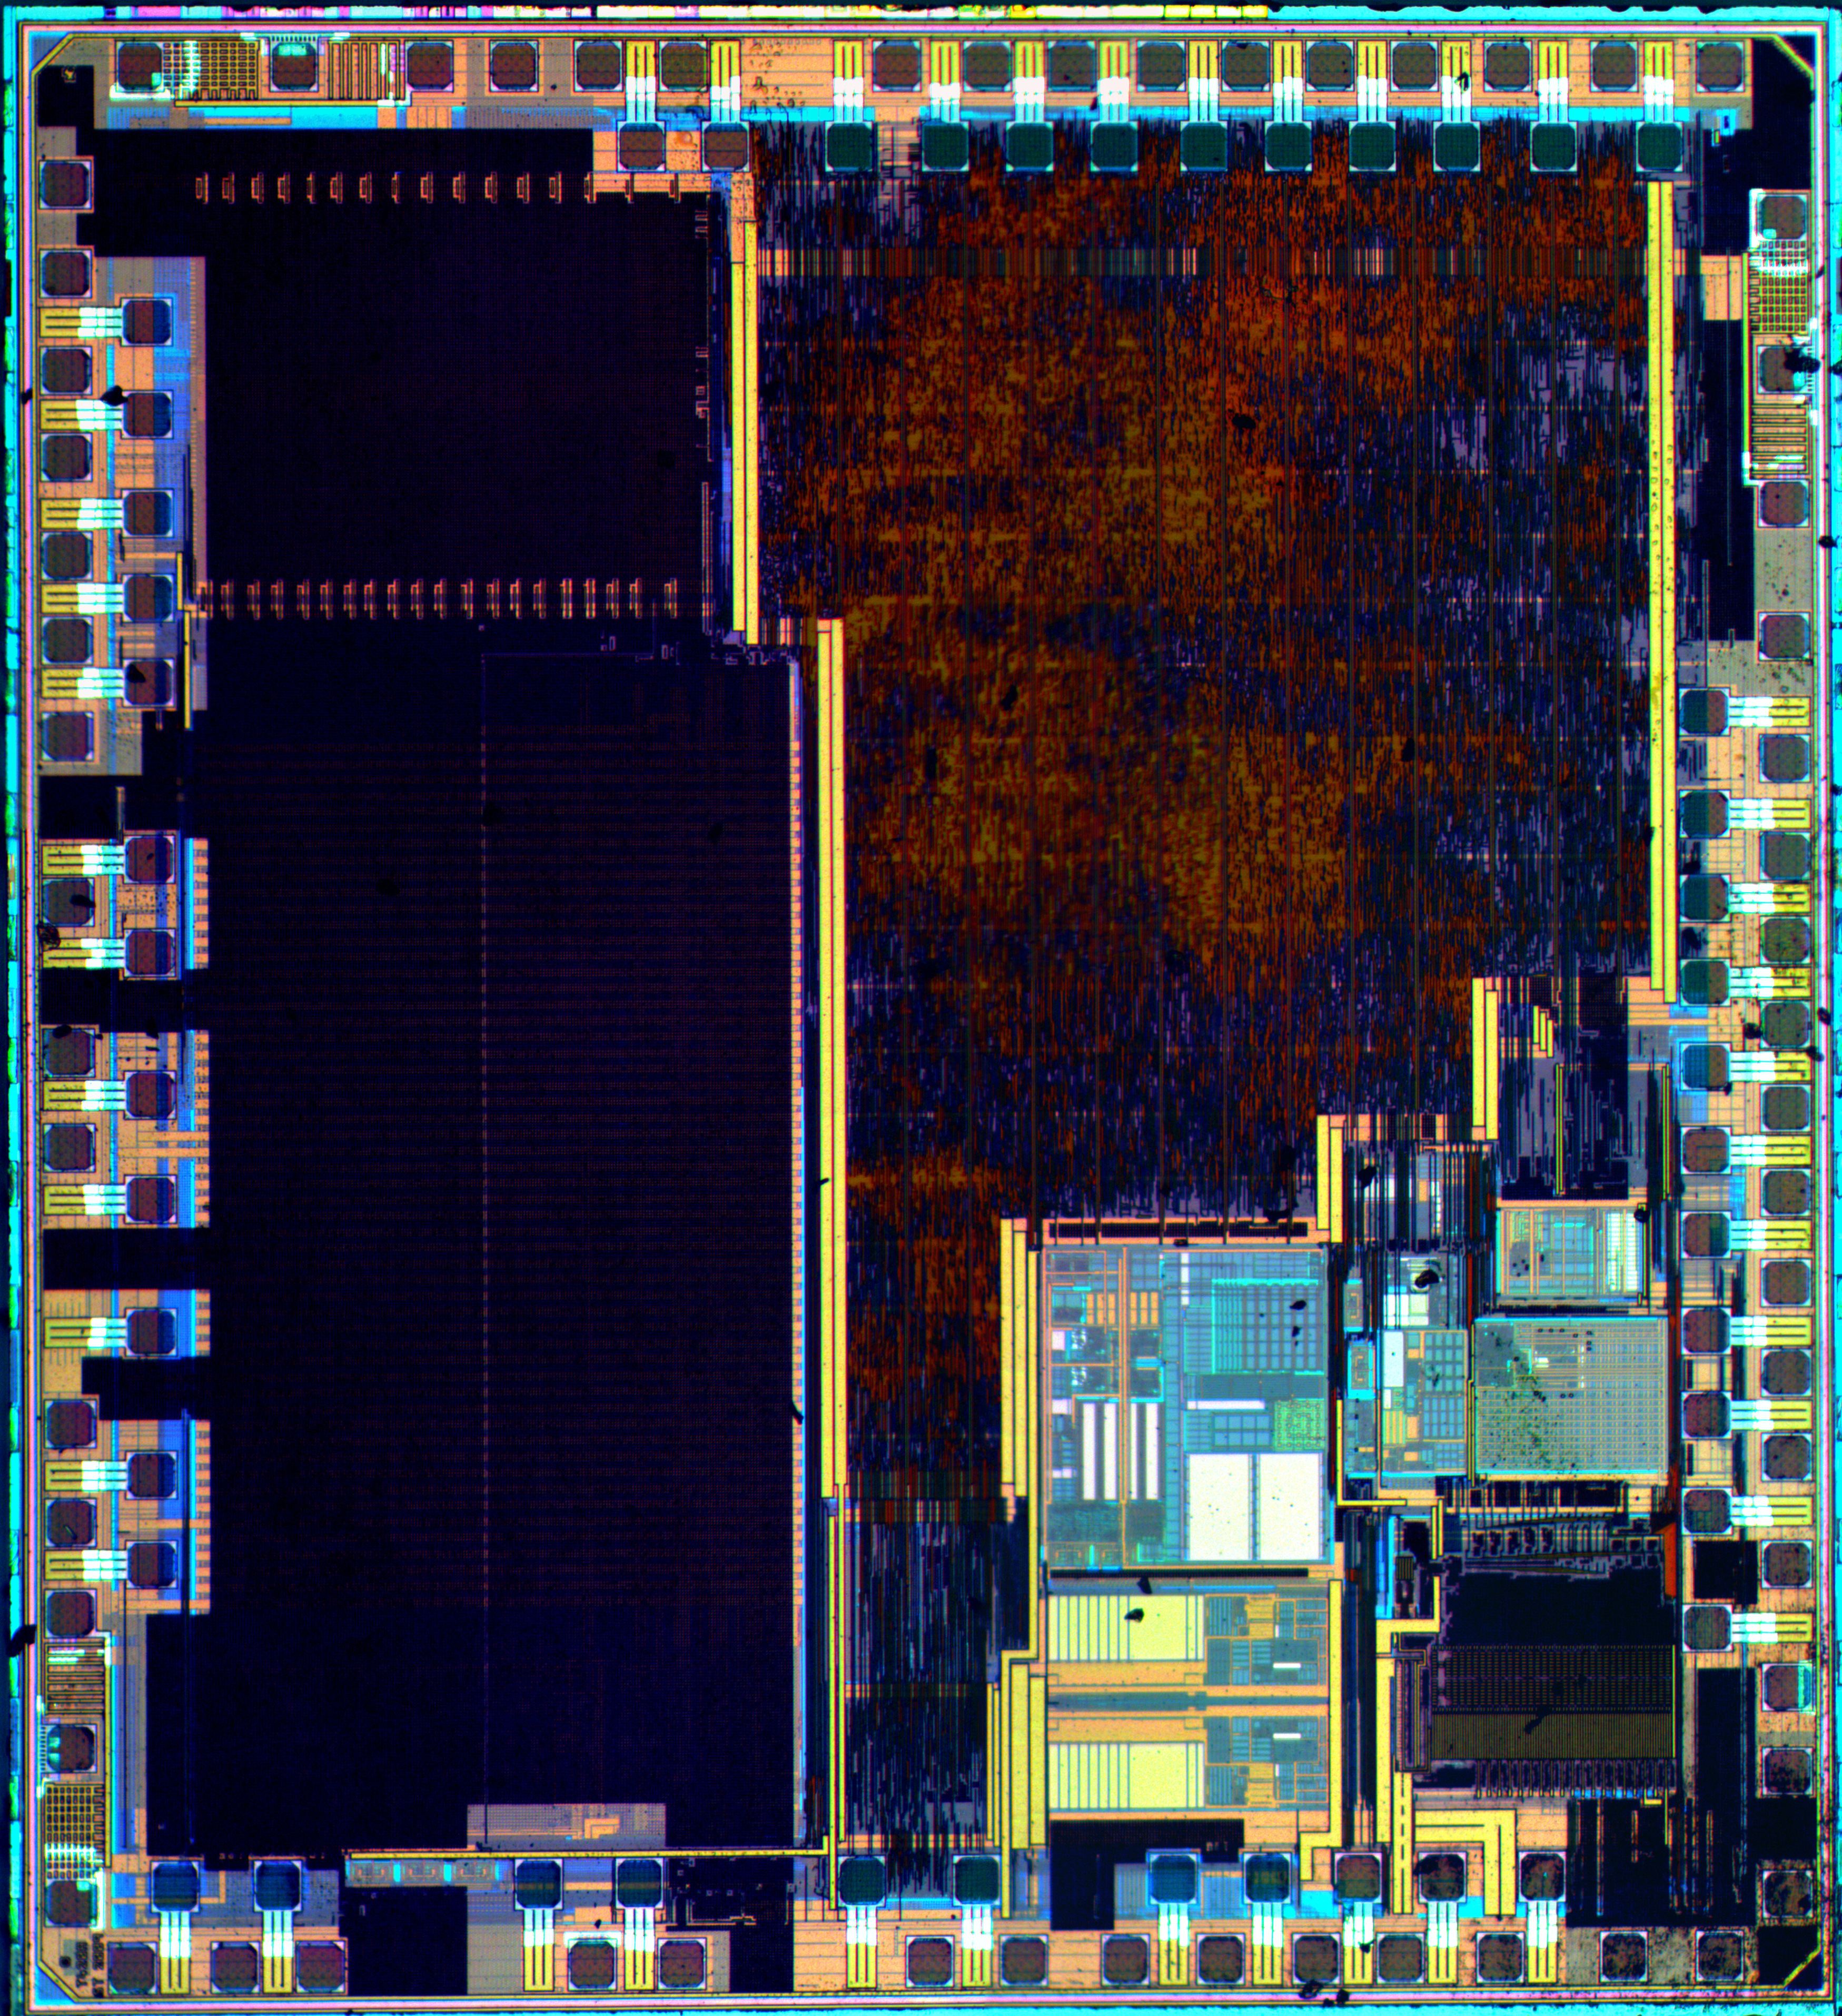
\includegraphics[width=0.8\textwidth]{resources/images/microcontroller.jpg}
    \caption[Mikrocontroller]{\enquote{bare chip} eines STM32F100C4T6B ARM Cortex-M3 microcontrollers\cite{microcontroller}}
    \label{fig:Microcontroller}
\end{figure}

Die Funktionsweise eines Mikrocontrollers beginnt mit der Bereitstellung eines Programms, das in den programmierbaren
Speicher geladen wird. Die \ac{CPU} interpretiert und führt die Anweisungen im Programm aus. Diese Anweisungen steuern die
Peripheriegeräte und verarbeiten die Daten gemäß den Anforderungen der Anwendung. Externe Eingangssignale können über
die \ac{GPIO}-Pins erfasst werden, während Ausgangssignale über dieselben Pins ausgegeben werden können.

\clearpage

Mikrocontroller finden in einer Vielzahl von Anwendungen Verwendung, darunter:
\begin{itemize}
    \item Automobilindustrie für Steuerungssysteme von Fahrzeugen.
    \item Haushaltsgeräte wie Mikrowellen, Waschmaschinen und Kühlschränke.
    \item Medizinische Geräte wie Blutzuckermessgeräte und Patientenüberwachungssysteme.
    \item Elektronische Spielzeuge und Unterhaltungselektronik.
    \item Industrielle Automatisierungssysteme zur Steuerung von Produktionsprozessen.
\end{itemize}
(Anwendungsorientierte Mikroprozessoren - Mikrocontroller und Digitale
Signalprozessoren\cite{Bähring2010})

\section{Serielle Schnittstellen}
Bei einer seriellen schnittstelle werden zur Datenübertragung einzelne Bits zeitlich nacheinander übertragen.
Damit steht diese Technik in Abgrenzung zu parallelen Schnittstellen, bei denen mehrere Bits auf mehreren
Stromkreisen zeitgleich übertragen werden.

Die Datenübertragung kann synchron oder asynchron erfolgen, bei synchroner Übertragung wird zu den
Datenleitungen noch eine Clock-Leitung benötigt, dass beide Geräte auf demselben Takt senden und empfangen
können. Bei asynchroner Übertragung müssen beide Geräte mit demselben internen Takt arbeiten und am Anfang
jeder Übertragung muss ein Synchronisations-Bit gesendet werden.

\begin{figure}[h]
    \centering
    \includegraphics[width=0.7\textwidth]{resources/images/Serial_and_Parallel_Data_Transmission.svg.png}
    \caption[Datenübertragungen]{Serielle und Parallele Datenübertragung gegenübergestellt \cite{ser-vs-par}}
    \label{fig:Seriell}
\end{figure}


Dazu gibt es unterschiedliche Übertragungs-Arten/Richtungen:
\begin{itemize}
    \item Simplex- oder Richtungsverkehr: \\
          Datenaustausch nur in eine Richtung
    \item Halb-Duplex- oder Wechselverkehr: \\
          Datenaustausch in beide Richtungen möglich, allerdings zeitlich versetzt
    \item Voll-Duplex- oder Gegenverkehr: \\
          Datenaustausch gleichzeitig in beide Richtungen
\end{itemize}

\begin{figure}[H]
    \centering
    \includegraphics[width=0.8\textwidth]{resources/images/Duplex.png}
    \caption[Varianten beim Datenaustausch]{Varianten beim seriellen Datenaustausch
        Samson - Serielle Datenübertragung \cite{seriell}[S.6]}
    \label{fig:Duplex}
\end{figure}

\subsection{RS-232}
RS-232 (Recommended Standard 232) ist ein Standard für eine asynchrone, serielle Schnittstelle und wurde
von dem US-amerikanischen Standardisierungsgremium Electronic Industries Association (EIA) entwickelt.

Die Datenleitungen arbeiten mit +12V Spannung als logische \enquote{0} und -12V als logische \enquote{1}.
Erlaubt sind aber auch jeweils Spannungen zwischen 5V und 15V. Diese Spannungspegel passen nicht zu
aktuellen \ac{TTL} Pegeln, daher werden heutzutage Treiberschaltkreise verwendet um, zwischen
\ac{TTL} - und RS-232 Pegeln zu wandeln.
\begin{figure}[H]
    \centering
    \includegraphics[width=1\textwidth]{resources/images/rs232_example.png}
    \caption[RS-232 Beispiel]{Beispielübertragung eines RS-232 Signals \cite{ser-example}}
    \label{fig:RS232}
\end{figure}

Es gibt eine \enquote{TxD} (Transmit Data) Leitung und eine \enquote{RxD} (Receive Data) Leitung, die
jeweils für das Senden und Empfangen von Daten (jeweils aus Sicht des \ac{DTE}) zuständig sind.
Damit handelt es sich um eine  Vollduplex-Verbindung, da ein zeitgleiches Senden und Empfangen möglich ist.

Obwohl der Standard keine festen Bitraten festlegt, wird in ihm darauf hingewiesen, dass er für
Übertragungsgeschwindigkeiten von bis zu 20 kbit/s gedacht ist. Typische \acp{UART}, die in Verbindung mit
RS-232 eingesetzt werden, unterstützen Übertragungsgeschwindigkeiten von 115,2 kbit/s oder sogar höher.

Um ein vorhersehbares Übertragungsverhalten sicherzustellen, legt die Norm eine maximale Flankensteilheit
für den Sender fest sowie eine minimale Flankensteilheit im Übergangsbereich von -3 V bis +3 V am Empfänger,
wobei diese von der gewählten Bitrate abhängig ist.
(Sprut - RS-232 \cite{rs232})

\subsection{1-Wire}
\label{sec:one_wire}

1-Wire ist eine serielle Schnittstelle der Firma Analog Devices. Außerdem ist 1-Wire auch eine
Spannungsschnittstelle mit Spannungen (anwendungsbabhängig) zwischen 2,8V und 6V. \\
Hierbei erfolgt die Energieversorgung der Slaves über die Datenleitung selbst: Während Zeiten geringer Aktivität (
Idle-Zustand) befindet sich die Datenleitung auf einem hohen Pegel (+3,3 V oder +5 V) und lädt dabei einen
in jedem 1-Wire-Slave integrierten Speicherkondensator auf (Parasite Power). Während der Kommunikation wird der
Bus von den Geräten (Devices) auf einen niedrigen Pegel gebracht. In diesen Phasen mit niedrigem Pegel wird der
Slave durch den Energievorrat seines Kondensators gespeist. Abhängig von seinem Ladestand kann der Kondensator
Low-Zeiten von bis zu etwa 960 \(\mu s\) überbrücken.

Das Bussystem ist nach dem One-Master/Multiple-Slaves-Prinzip aufgebaut, d.h. es gibt einen Master (Steuereinheit),
der die Kommunikation mit den Slaves (Sensoren, Aktoren) steuert. Die bis zu 100 Slaves können nicht untereinander
kommunizieren.\\
Jeder dieser Slaves wird durch eine eindeutige 64-Bit-Adresse adressiert, die sich durch eine 8-Bit-Familiennummer,
eine 48-Bit-Seriennummer und eine 8-Bit-Prüfsumme zusammensetzt. Die 8-Bit-Familiennummer ist eine Kennung für
die Art des Slaves, die 48-Bit-Seriennummer ist eine eindeutige Kennung für den Slave und die 8-Bit-Prüfsumme
dient zur Fehlererkennung.

Die Datenübertragung erfolgt über eine einzige Datenader, die gleichzeitig als Strom-, Sende- und Empfangsleitung
genutzt wird. Der Bus funktioniert Halbduplexverfahren und asynchron, da es keine eigene Timerleitung gibt.
Die Synchronisation erfolgt bei jedem Bit über der vom Master erzeugten fallenden Flanke.
\renewcommand{\arraystretch}{2}%
\begin{table}[ht]
    \centering
    \begin{tabularx}{\textwidth}{|l|X|X|}
        \hline
        \textbf{Operation} & \textbf{Beschreibung}                                                          & \textbf{Implementierung} \\
        \hline
        Write 1 bit        & Sendet ein '1'-Bit an die 1-Wire-Slaves (Schreibzeitfenster 1)                 &
        Bus auf Low ziehen, Verzögerung A Bus freigeben, Verzögerung B                                                                 \\
        \hline
        Write 0 bit        & Sendet ein '0'-Bit an die 1-Wire-Slaves (Schreibzeitfenster 0)                 &
        Bus auf Low ziehen, Verzögerung C Bus freigeben, Verzögerung D                                                                 \\
        \hline
        Read bit           & Liest ein Bit von den 1-Wire-Slaves (Lesezeitfenster)                          &
        Bus auf Low ziehen, Verzögerung A Bus freigeben, Verzögerung E
        Bus abtasten, um das Bit vom Slave zu lesen Verzögerung F                                                                      \\
        \hline
        Reset              & Setzt die 1-Wire-Bus-Slave-Geräte zurück und bereitet sie für einen Befehl vor &
        Verzögerung G Bus auf Low ziehen, Verzögerung H Bus freigeben,
        Verzögerung I Bus abtasten, 0 = Gerät(e) vorhanden, 1 = kein Gerät vorhanden
        Verzögerung J                                                                                                                  \\
        \hline
    \end{tabularx}
    \caption{Übersicht der 1-Wire-Bus-Operationen und deren Implementierung.}
    \label{tab:1wire_operations}
\end{table}

\begin{figure}[H]
    \centering
    \includegraphics[width=1\textwidth]{resources/images/onewire.png}
    \caption[1-Wire Beispiel]{1-Wire Übertragung Wellenformen \cite{1wire}}
    \label{fig:1w}
\end{figure}

\renewcommand{\arraystretch}{1}
\begin{table}[H]
    \centering
    \begin{tabular}{|c|c|c|}
        \hline
        \textbf{Parameter} & \textbf{Standard (\(\mu s\))} & \textbf{Overdrive (\(\mu s\))} \\
        \hline
        A                  & 6                             & 1.0                            \\
        B                  & 64                            & 7.5                            \\
        C                  & 60                            & 7.5                            \\
        D                  & 10                            & 2.5                            \\
        E                  & 9                             & 1.0                            \\
        F                  & 55                            & 7                              \\
        G                  & 0                             & 2.5                            \\
        H                  & 480                           & 70                             \\
        I                  & 70                            & 8.5                            \\
        J                  & 410                           & 40                             \\
        \hline
    \end{tabular}
    \caption{Übersicht der Empfohlenen Verzögerungs Werte.}
    \label{tab:standard_overdrive}
\end{table}

Für das Setzen einer logischen 1 zieht der Master den Bus für 1 bis 15 \(\mu s\) auf einen Low-Pegel, während er für eine
logische 0 den Bus für 60 bis 120 \(\mu s\) auf Low hält. Beim Lesen zieht der Master, ähnlich wie bei der \enquote{Write 1}-Signalisierung,
den Bus für 1 bis 15 \(\mu s\) auf einen Low-Pegel, während der Slave den Bus für die Übertragung einer logischen 0 zusätzlich auf
Low hält. Für einen Reset sendet der Master einen Low-Pegel-Impuls mit einer Dauer von 480 \(\mu s\). Ein Slave signalisiert seine
Präsenz, indem er den Bus innerhalb von 60 \(\mu s\) nach dem Reset für mindestens 60 \(\mu s\) auf Low zieht.

Die 1-Wire-Geräte unterstützen außerdem einen Overdrive-Modus, der die Möglichkeit bietet, deutlich höhere Übertragungsraten
zu erreichen. Im Overdrive-Modus reicht es für eine logische 1 aus, den Bus lediglich für 1–2 \(\mu s\) auf einen Low-Pegel zu ziehen,
während 6 \(\mu s\) für eine logische 0 im Overdrive-Modus ausreichend sind. Ein Reset kann bereits in 48 \(\mu s\) erzeugt werden.
Wenn das Reset-Signal länger als 80 \(\mu s\) ist, schalten die 1-Wire-Geräte in den regulären Betriebsmodus, ansonsten bleiben
sie im Overdrive-Modus.

Im regulären Betriebsmodus ermöglichen die oben genannten Timing-Bedingungen Datenraten von bis zu 16,3 KBit/s.
Durch den Overdrive-Modus kann diese Geschwindigkeit auf bis zu 142 KBit/s gesteigert werden.
(Analog - 1-Wire \cite{1wire})

\subsection{\Ac{USB}}
Bei \ac{USB} handelt es sich um eine weltweit etablierte Schnittstelle, die zur Verbindung verschiedener
elektronischer Geräte dient. Es gibt diverse standardisierte Stecker und Buchsen, außerdem gibt es verschiedene
\ac{USB}-Standards, die sich in der Übertragungsgeschwindigkeit und der maximalen Stromstärke unterscheiden.
Die Übertragung erfolgt dabei meist über vier Adern, zwei für die Datenübertragung und zwei für die Stromversorgung.
Erst bei dem Standard USB 3.0 wurde die Anzahl der Datenleitungspaare erhöht, um die Übertragungsgeschwindigkeit durch
mehrere serielle Übertragungen parallel zueinander zu erhöhen.
\begin{figure}[H]
    \centering
    \includegraphics[width=0.5\textwidth]{resources/images/usb.png}
    \caption[\ac{USB} Stecker]{\ac{USB} Stecker Auswahl\cite{usb}}
    \label{fig:usb}
\end{figure}
Elektrisch gesehen ist \ac{USB} eine direkte Verbindung zwischen zwei Geräten. Die Bus Eigenschaft wird erst oberhalb der
physikalischen Schicht durch das \ac{USB}-Protokoll erreicht. Ein Host-Controller(Master) verwaltet dabei die angeschlossenen
Peripheriegeräte(Slaves). An einen \ac{USB}-Port kann immer nur ein einzelnes \ac{USB}-Gerät angeschlossen werden. Um das
theoretische Maximum von 127 Geräten zu erreichen, werden \ac{USB}-Hubs verwendet. Diese werden an einen \ac{USB}-Port
angeschlossen und stellen mehrere \ac{USB}-Ports zur Verfügung. Die Kommunikation mit den angeschlossenen Geräten wird dabei
vom Host-Controller übernommen.

\subsection{\Ac{CAN} Bus}
\ac{CAN} ist ein asynchrones, serielles Bussystem, das ursprünglich für die Automobilindustrie entwickelt wurde.
Die Datenübertragung in einem \ac{CAN}-Bus basiert auf einem speziellen Kommunikationsprotokoll,
das es ermöglicht, zuverlässig und effizient Daten zwischen verschiedenen \acp{ECU} zu übertragen.
Hier ist eine Erklärung der Datenübertragung im \ac{CAN}-Bus:

Die Datenübertragung im \ac{CAN}-Bus erfolgt mithilfe von Frames, die verschiedene Typen haben:
\begin{itemize}
    \item \textbf{Data Frame}: Enthält die tatsächlichen Nutzdaten, die zwischen \acp{ECU} ausgetauscht werden sollen.
    \item \textbf{Remote Frame}: Wird verwendet, um von einem ECU Daten anzufordern, ohne sie tatsächlich zu senden.
    \item \textbf{Error Frame}: Wird verwendet, um Fehlerzustände zu signalisieren.
    \item \textbf{Overload Frame}: Signalisiert, dass der Empfänger vorübergehend überlastet ist und keine neuen Frames
          empfangen kann.
\end{itemize}

Ein typischer Data Frame im \ac{CAN}-Bus besteht aus folgenden Teilen:
\begin{itemize}
    \item \textbf{Start-of-Frame (SOF)}: Ein spezielles Bit, das den Beginn eines neuen Frames anzeigt.
    \item \textbf{Arbitrierungsfeld}: Enthält den Identifier des Frames, der verwendet wird, um die Priorität der
          Nachrichten zu bestimmen.
    \item \textbf{Control-Feld}: Enthält Informationen über die Länge der Nutzdaten und den Frame-Typ.
    \item \textbf{Datenfeld}: Hier werden die eigentlichen Nutzdaten übertragen.
    \item \textbf{CRC-Feld}: Enthält eine Prüfsumme, die zur Fehlererkennung verwendet wird.
    \item \textbf{ACK-Feld}: Wird von Empfängern verwendet, um den erfolgreichen Empfang des Frames zu bestätigen.
    \item \textbf{End-of-Frame (EOF)}: Ein spezielles Bit, das das Ende des Frames anzeigt.
\end{itemize}

Wenn mehrere \acp{ECU} gleichzeitig Daten senden möchten, nutzt der \ac{CAN}-Bus eine Arbitrierungsmethode, um zu entscheiden,
welcher Frame Vorrang hat. Dies geschieht durch Bit-Arbitrierung, bei der \acp{ECU} die gesendeten Bits überwachen und abbrechen,
wenn sie feststellen, dass ihre gesendete Bitfolge mit einer anderen kollidiert.

Der \ac{CAN}-Bus verwendet eine CRC-Prüfsumme, um die Integrität der empfangenen Daten zu überprüfen.
Empfänger vergleichen die empfangene Prüfsumme mit der berechneten Prüfsumme, um festzustellen, ob Fehler aufgetreten sind.
Wenn ein Fehler erkannt wird, wird der Frame von den Empfängern abgelehnt.

Die Datenübertragung im \ac{CAN}-Bus ermöglicht zuverlässige und robuste Kommunikation zwischen \acp{ECU} in anspruchsvollen
Umgebungen wie Fahrzeugen, Industrieanlagen und anderen Anwendungen. Das Protokoll sorgt dafür, dass Daten korrekt
übertragen und priorisiert werden, während gleichzeitig Fehler erkannt und behandelt werden können.

\section{iButton\textregistered}

\begin{wrapfigure}{r}{0.40\textwidth}
    \centering
    \includegraphics[width=0.35\textwidth]{resources/images/product-ibutton.jpg}
    \caption[iButton]{typische iButton Anwendung\cite{iButtonPic}}
    \label{fig:iButton}
\end{wrapfigure}

iButton\textregistered\ ist ein Produkt der Firma Analog Devices. Dabei handelt es sich um einen integrierten
Schaltkreis in einem Zylindrischen Edelstahlgehäuse, der über das 1Wire-Protokoll kommuniziert. \\
Jedes iButton Gerät hat eine weltweit einzigartige  64-bit-Seriennummer (bestehend aus 8-Bit Family Code,
48-Bit Nummer (Unique Device ID) und 8-Bit Zyklische-Redundanzprüfungs Prüfsumme).\\
(Analog Devices - iButton\cite{iButton})

\section{Gleichspannungswandler}

Bei Gleichspannungs- oder auch DC-DC-Wandlern handelt es sich um elektrische Schaltungen, welche die am Eingang
anliegende Gleichspannung in eine Gleichspannung mit höherem, niedrigerem oder invertiertem Spannungsniveau am
Ausgang umwandelt. \\
Dies geschieht durch einen periodisch arbeitenden Schalter und einen oder mehrere Energiespeicher.

\subsection{Buck}
Der Buck-Wandler oder auch Abwärtswandler ist ein schaltender Gleichspannungswandler, der eine höhere
Eingangsspannung \(U_E\) in eine niedrigere Ausgangsspannung \(U_A\) umwandelt.

\begin{figure}[H]
    \centering
    \includegraphics[width=0.7\textwidth]{resources/images/Buck_operating.svg.png}
    \caption[Buck]{Buck Wandler\cite{buck}}
    \label{fig:buck}
\end{figure}

\begin{figure}[H]
    \centering
    \includegraphics[width=0.9\textwidth]{resources/images/Tiefsetzsteller_Funktion.png}
    \caption[Buck Spannungen]{Buck Wandler - Spannungsverlauf\cite{buck2}}
    \label{fig:buck_waveforms}
\end{figure}

Das konzeptionelle Modell des Abwärtswandlers lässt sich am besten anhand des Verhältnisses zwischen Strom
und Spannung der Spule verstehen. \\
Zu Beginn, wenn der Schalter offen ist (Aus-Zustand), ist der Strom im
Stromkreis gleich Null. Wenn der Schalter zum ersten Mal geschlossen wird (Ein-Zustand), beginnt der Strom
zu steigen und die Induktivität erzeugt als Reaktion auf den sich ändernden Strom eine entgegengesetzte
Spannung an ihren Anschlüssen. Dieser Spannungsabfall wirkt der Spannung der Quelle entgegen und verringert
somit die Nettospannung an der Last. \\
Mit der Zeit nimmt die Änderungsrate des Stroms ab und die Spannung an der Induktivität sinkt ebenfalls,
wodurch die Spannung an der Last steigt. Während dieser Zeit speichert die Induktivität Energie in Form
eines Magnetfelds.

Wenn der Schalter geöffnet wird, während sich der Strom noch ändert, kommt es immer zu einem Spannungsabfall
über der Induktivität, so dass die Nettospannung an der Last immer kleiner ist als die Eingangsspannung der
Quelle. Wenn der Schalter wieder geöffnet wird (Aus-Zustand), wird die Spannungsquelle aus dem Stromkreis
entfernt, und der Strom nimmt ab. Der abnehmende Strom erzeugt einen Spannungsabfall an der Induktivität
(im Gegensatz zum Anstieg im Ein-Zustand), und die Induktivität wird nun zu einer Stromquelle. \\
Die gespeicherte Energie im Magnetfeld der Induktivität unterstützt den Stromfluss durch die Last.
Dieser Strom, der bei abgeschalteter Eingangsspannung fließt, summiert sich mit dem Strom, der im
Ein-Zustand fließt, zu einem Strom, der größer ist als der durchschnittliche Eingangsstrom.

Durch den Kondensator wird die sägezahnförmige Ausgangsspannung geglättet und die Spannungsspitzen 
werden abgeflacht. 

Der Schalter schaltet zwischen Ein- und Aus-Zustand hin und her, um die Spannung an der Last zu regeln.
Dabei wird das Verhältnis zwischen Ein- und Aus-Zeit wird als Tastverhältnis \(d\) bezeichnet.
\[\displaystyle d = \frac{T_e}{T}\]
Mit idealen Bauteilen und ohne Verluste gilt für die Ausgangsspannung:
\[U_a = U_e \times d\]

\subsection{\ac{SEPIC}}
Ein \ac{SEPIC} Wandler ein Gleichspannungswandler, bei dem die Eingangsspannung sowohl größer, als auch
kleiner als die Ausgangsspannung sein kann.

\begin{figure}[H]
    \centering
    \includegraphics[width=\textwidth]{resources/images/sepic.png}
    \caption[SEPIC Wandler]{schematische Darstellung \\ eines SEPIC Wandlers}
    \label{fig:SEPIC}
\end{figure}

Die schematische Darstellung eines grundlegenden SEPIC ist in Abbildung \ref{fig:SEPIC} zu sehen. Wie bei anderen
Schaltnetzteilen (insbesondere Gleichspannungswandlern) wird auch beim SEPIC Energie zwischen den Kondensatoren
und Induktivitäten geschaltet, um eine Spannung in eine andere umzuwandeln. Die Menge der ausgetauschten Energie
wird durch den Schalter Q1 gesteuert, bei dem es sich in der Regel um einen Transistor wie z. B. einen \ac{MOSFET}
handelt. \\
Das Verhältniss zwischen ein- und ausgeschaltetem Schalter Q1 wird dabei \enquote{Duty cycle} genannt und wird
(bei Annahme von 100\% Effizienz) durch die folgende Formel berechnet:

\[\displaystyle D = \frac{V_{OUT} + V_{FWD}}{V_{IN} + V_{OUT} + V_{FWD}}\]

\begin{itemize}
    \item \(V_{IN}\)  ist die Eingangsspannung
    \item \(V_{OUT}\) ist die Ausgangsspannung
    \item \(V_{FWD}\) ist die Durchlassspannung der Diode D1
\end{itemize}

Der Maximale Duty cycle D tritt bei der kleinsten Eingangsspannung auf und entsprechend ist der minimale
Duty cycle bei der größten Eingangsspannung.

\begin{figure}[H]
    \centering
    \includegraphics[width=0.9\textwidth]{resources/images/sepic_schalter.png}
    \caption[SEPIC Spannungen]{SEPIC Wandler - Schalterzustände}
    \label{fig:SEPIC_Schalter}
\end{figure}

Wenn der Schalter Q1 eingeschaltet wird, steigt der Strom \(I_{L1a}\) und der Strom \(I_{L1b}\) 
wird negativer. Die Energie zur Erhöhung des Stroms \(I_{L1a}\) kommt von der Eingangsquelle. 
Da Q1 kurzzeitig geschlossen ist und die momentane Spannung \(V_{L1a}\) ungefähr \(V_{in}\) 
beträgt, ist die Spannung \(V_{L1b}\) ungefähr \(- V_{Cp}\). Daher wird D1 geöffnet und der 
Kondensator C1 liefert die Energie, um die Stromstärke in \(I_{L1b}\) zu erhöhen und somit 
die in L2 gespeicherte Energie zu steigern. IL wird von C2 gespeist. Am einfachsten lässt 
sich dies veranschaulichen, wenn man die Vorspannungen der Schaltung im Gleichstromzustand 
betrachtet und dann Q1 schließt.

Wenn der Schalter Q1 ausgeschaltet wird, entspricht der Strom \(I_{Cp}\) dem Strom \(I_{L1a}\), 
da Induktivitäten keine sofortigen Stromänderungen zulassen. Der Strom \(I_{L1b}\) fließt weiterhin 
in negativer Richtung, er kehrt seine Richtung nie um. Aus dem Diagramm ist ersichtlich, dass sich 
ein negativer \(I_{L1b}\) zum Strom \(I_{L1a}\) addiert und den an die Last abgegebenen Strom erhöht. 
Mit Hilfe des Kirchhoffschen Stromgesetzes kann gezeigt werden, dass \(I_{D1} = I_{Cp} - I_{L_1b}\) ist. 
Daraus lässt sich schließen, dass, während Q1 ausgeschaltet ist, die Last sowohl von L2 als auch 
von L1 mit Strom versorgt wird. C1 wird jedoch während dieses Aus-Zyklus von L1 geladen 
(genauso, wie C2 von L1 und L2) und wird L2 während des folgenden Ein-Zyklus wieder aufladen. \\ 
Die Ausgangsspannung \(V_{OUT}\) lässt soch Folgendermaßen berechnen:
\[U_A = \frac{D}{1 - D} \times U_E\]
(Texas Instruments - Designing DC/DC converters based on \ac{SEPIC} topology \cite{sepic}) \\
(Ulrich Schlienz - Schaltnetzteile und ihre Peripherie \cite{Schlienz2020}(ab S. 61))
